
\documentclass[
               letterpaper,%|a4paper|a5paper|b5paper|legalpaper|executivepaper,
               10pt,%|11pt|12pt,
               oneside,%|twoside,
               onecolumn,%|twocolumn,
               final,%|draft,
               openany%|openright
              ]{report}
% Die folgenden Pakete erleichtern die Verwendung der deutschen Sprache deutlich
\usepackage[utf8]{inputenc}
\usepackage{graphicx}
\usepackage{listings}
\usepackage{xcolor}
\colorlet{punct}{red!60!black}
\definecolor{background}{HTML}{EEEEEE}
\definecolor{delim}{RGB}{20,105,176}
\colorlet{numb}{magenta!60!black}
\lstdefinelanguage{json}{
    basicstyle=\normalfont\ttfamily,
    numbers=left,
    numberstyle=\scriptsize,
    stepnumber=1,
    numbersep=8pt,
    showstringspaces=false,
    breaklines=true,
    frame=lines,
    backgroundcolor=\color{background},
    literate=
     *{0}{{{\color{numb}0}}}{1}
      {1}{{{\color{numb}1}}}{1}
      {2}{{{\color{numb}2}}}{1}
      {3}{{{\color{numb}3}}}{1}
      {4}{{{\color{numb}4}}}{1}
      {5}{{{\color{numb}5}}}{1}
      {6}{{{\color{numb}6}}}{1}
      {7}{{{\color{numb}7}}}{1}
      {8}{{{\color{numb}8}}}{1}
      {9}{{{\color{numb}9}}}{1}
      {:}{{{\color{punct}{:}}}}{1}
      {,}{{{\color{punct}{,}}}}{1}
      {\{}{{{\color{delim}{\{}}}}{1}
      {\}}{{{\color{delim}{\}}}}}{1}
      {[}{{{\color{delim}{[}}}}{1}
      {]}{{{\color{delim}{]}}}}{1},
}

\graphicspath{ {./img/} }

\usepackage[T1]{fontenc} % Wird u.a. f\"ur das Trennen von W\"ortern 
                         % mit Umlauten genutzt.
\usepackage{ngerman} % Wird ben\"otigt um deutsche Bezeichnungen zu
                     % erhalten. Zum Beispiel Inhaltsverzeichnis anstelle
                     % von Table of contents.  
                     % Auch werden dann die W\"orter gem\"a\ss{} der neuen
                     % Rechtschreibung getrennt. 

% Titelseite beziehungsweise der Inhalt derselbigen:
\title{Verteilte Systeme Labor Aufgabe 2}
\author{Adrian Häuser 71141 haad1014@hs-karlsruhe.de,\\ Tom Ganz 71127 tomganzka@gmail.com}
% als Datum wird automatisch das aktuelle Datum gesetzt


\begin{document}
\maketitle


\tableofcontents % Inhaltsverzeichnis

\chapter{Die Architektur}

\begin{figure}[h!]
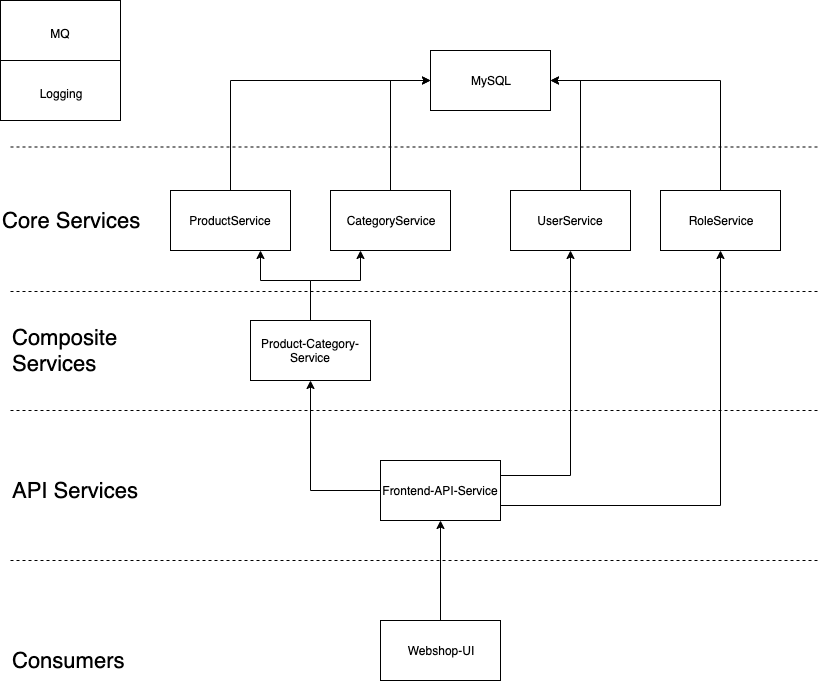
\includegraphics[scale=0.4]{api}
\caption{Die verteilte Microservice Architektur}
\label{fig:arch}
\centering
\end{figure}
Wie in Abbildung \ref{fig:arch} zu erkennen, haben wir die Anwendung in vier Coreservices unterteilt, eine für jedes DAO der Legacy-Anwendung. Diese führen CRUD Operationen auf einer gemeinsamen Datenbank-Server aus, auf dem sich für jeden Coreservice eine Datenbank befindet. Ein Composite Service existiert, welcher Eigenschaften wie referenzielle Integrität erzwingt für Productservice und CategoryService. Der API-Service stellt wiederum ein einziges Interface für die Webshop-UI zur Verfügung.\\
Falls am Ende Kapazitäten von unserer Seite zur Verfügung stehen, wird ein globaler Logging-Service implementiert, welcher über eine Message Queue z.B. Apache Kafka Nachrichten entgegennimmt und persistiert.


\chapter{Swagger-Schemata}
\begin{figure}[h!]
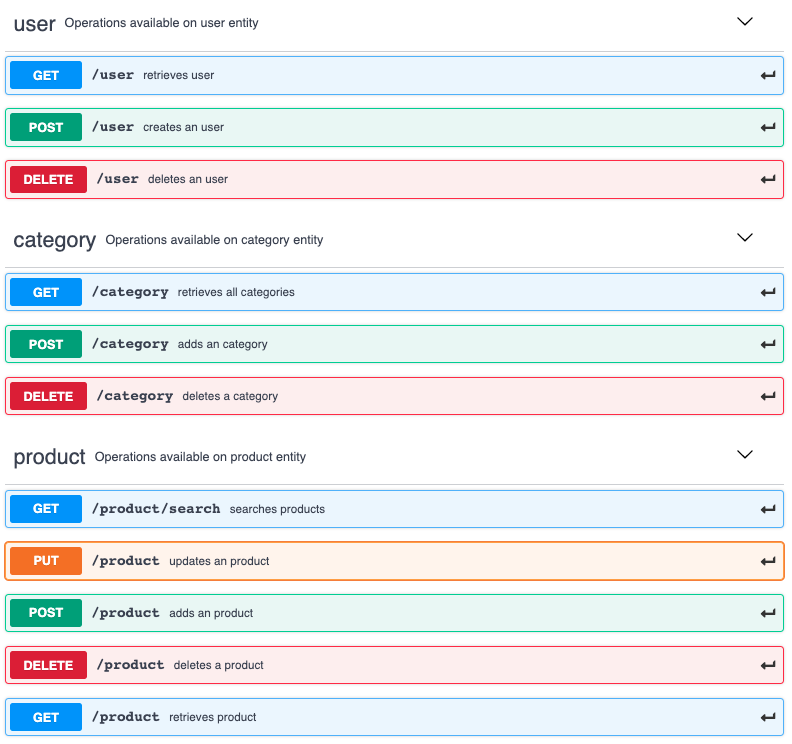
\includegraphics[scale=0.4]{schema1}
\caption{Die Endpunkte definiert durch Swagger}
\label{fig:schema1}
\centering
\end{figure}
In Abbildung \ref{fig:schema1} sind die von uns spezifizierten Endpunkte und ihre Beschreibungen zu sehen. 
\begin{figure}[h!]
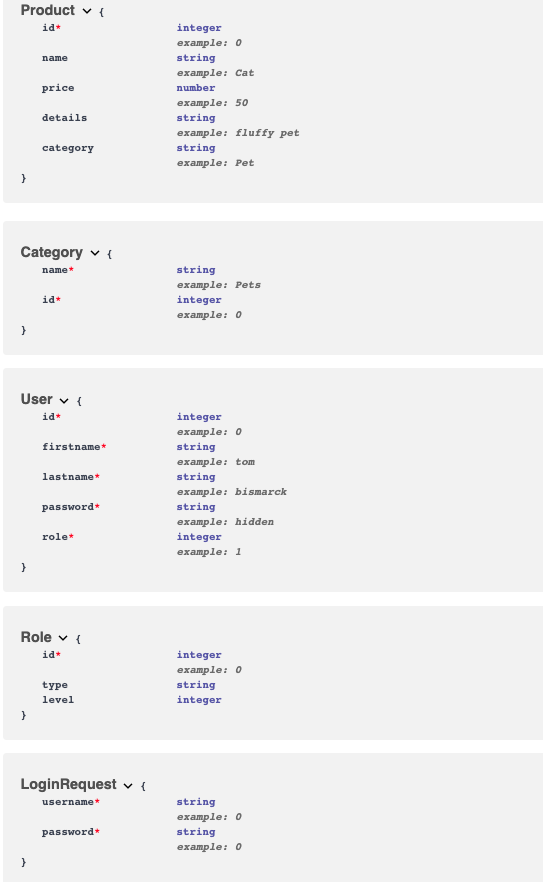
\includegraphics[scale=0.5]{schema2}
\caption{Die Models definiert durch Swagger}
\label{fig:schema2}
\centering
\end{figure}
In Abbildung \ref{fig:schema2} sind die Modelle, die für die Eingabe und Ausgabe gebraucht werden definiert.
\end{document}   